\title{Local Search}
\label{chp:local-search}
\author{Sara Ceschia, Luca Di Gaspero, Andrea Schaerf}
\institute{DPIA, University of Udine\\ 
\texttt{\{sara.ceschia,luca.digaspero,andrea.schaerf\}@uniud.it}}
\maketitle


\emph{Local Search} is an algorithmic paradigm for combinatorial
search and optimization, which has been shown to be very effective for many
problems in the scientific literature. A large number
of techniques based on local search have been proposed to successfully
address a variety of practical problems.


Local search techniques belong to the larger class of the so-called
\emph{selective} methods that are based on the exploration of the
search space composed by complete solutions. This is opposed to
\emph{constructive} methods that build the solution in a step-by-step
manner by iteratively adding a new piece to the partial solution constructed
that far.  

In addition, local search techniques are non-exact, as they
do not guarantee to find the optimal solution. In the cases in which
the optimal solution is found, there is no way to prove that it is
indeed optimal, unless it has been established
with exact techniques that it is not possible to reach a value lower than that (i.e., it is a proven \emph{lower bound}).

Local search is based on the simple idea of \emph{navigating} the
search space by iteratively stepping from one state to one of its
\emph{neighbors}. The neighborhood of a state is the set of states
that can be obtained by applying a ``local change'' to it. The
definition of the neighborhood relation is dependent on the specific
problem under consideration, although there are some common
patterns that can be applied to search spaces with
similar structure.  The mechanism upon which the neighbor is selected
at each step is one of the main design choices that varies
among different local search techniques. In any case, this selection
mechanism relies upon the definition of the \emph{cost function} $F$,
which assesses the quality of each neighbor state, and it is also
problem dependent.

% NEW PARAGRAPH
Even though it is difficult to assess precisely when local search should be 
used instead of other optimization methods, a general observation is that 
its behavior depends on the landscape of the cost function. More precisely, if the 
landscape is relatively \emph{smooth} with respect to local 
changes, it is more likely that local search techniques will be successful.


In this chapter, we discuss the key elements of the local
search paradigm, which are independent of both the specific problem 
and the specific local search technique chosen to solve it.

We also introduce the basic local search techniques and discuss some
improvements and variations of such basic methods. We refer to
the following chapters %Chapter~\ref{cap:simulated-annealing} 
and the book by Hoos and St\"utzle \cite{HoSt05} for more complex local search
techniques. % others?



\section{Local Search Elements}

We first introduce one by one the key elements of local search.  In
detail, we will introduce the notions of \emph{search space},
\emph{neighborhood relation}, \emph{cost function}, \emph{initial
  solution selection}, \emph{move selection and acceptance criterion},
and \emph{stop criterion}.

\subsection{Search Space}

Given a search or optimization problem $P$ and an instance $I$ of $P$, we
associate to it a search space $S$, with the following properties:

\begin{itemize}
\item each element $s\in S$ represents a solution of $I$, not
  necessarily feasible (i.e., it might violate some constraint of the problem);
\item for search problems, at least one feasible solution of $I$ is
  represented in $S$;
\item for optimization problems, at least one optimal solution of $I$
  is represented in $S$.
\end{itemize}

If the previous requirements are met, we have a \emph{valid
  representation} of the problem. We refer to an element $s\in S$ as a
\emph{state}.

% Q: is n-queens already defined?
Consider for example the classical $n$-queens problem, which consists
in placing $n$ queens in an $n\times n$ chessboard so that they do not
attack each other neither vertically, nor horizontally, nor diagonally.

The direct representation of the problem would be with an $n\times n$
matrix of boolean-values, each representing the presence/absence of a
queen in the corresponding square. However, the intuitive search
spaces for local search already partition the chessboard in columns,
making use of $n$ integer-valued variables $\mathbf{x} = [x_1, x_2,
\dots, x_n]$ such that the assignment $x_i = j$ corresponds to place a
queen in position $(j,i)$ in the chessboard. Since this representation
places only one queen in each column, it implicitly provides against
vertical attacks.

There are two typical options for the definition of the
search space for the $n$-queens problem:

\begin{itemize}
\item \textbf{Assignment}: any variable $x_1,\dots, x_n$ can assume
  any value in the domain $\chi = \{1,\dots,n\}$. 
\item \textbf{Permutation}: variables can assume only distinct values in the domain $\chi = \{1,\dots,n\}$, resulting in a permutation of the numbers $1,\dots,n$. 
\end{itemize}

For example, $\mathbf{s_1} = [4,6,1,6,8,4,2,1]$ is a state for the instance with
$n = 8$ for \textbf{Assignment}, and $\mathbf{s_2} = [4,1,7,6,8,3,2,5]$ is a
state for both search spaces. These states are depicted in Figures~\ref{fig:nqueens-assignment} and \ref{fig:nqueens-permutation}.
% replace il the figure X with s_1 and s_2 (LUCA)

\begin{figure}
  \subfigures 
  \begin{minipage}{\textwidth}
    \leftfigure[t]{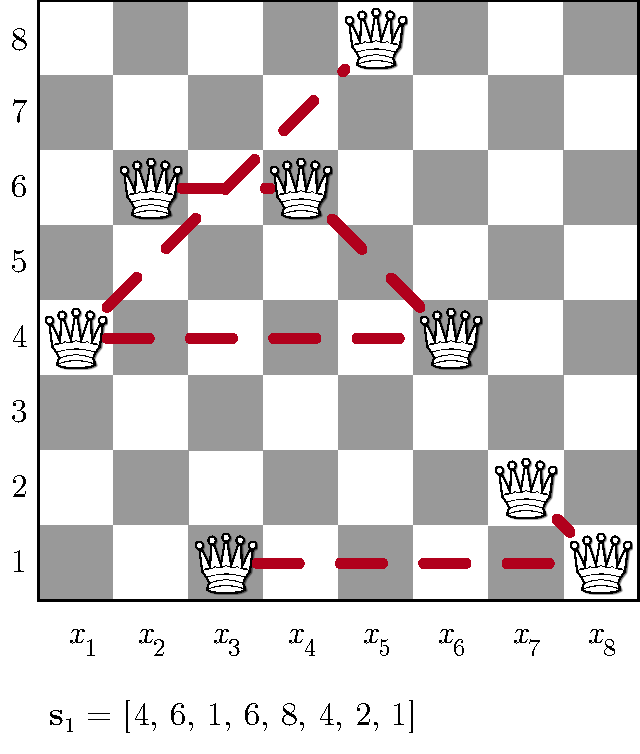
\includegraphics[width=0.4\textwidth]{"Part 2 - Search-Based Optimization/Local Search/n-queens/assignment.pdf"}}
    \hspace{\fill}
    \rightfigure[t]{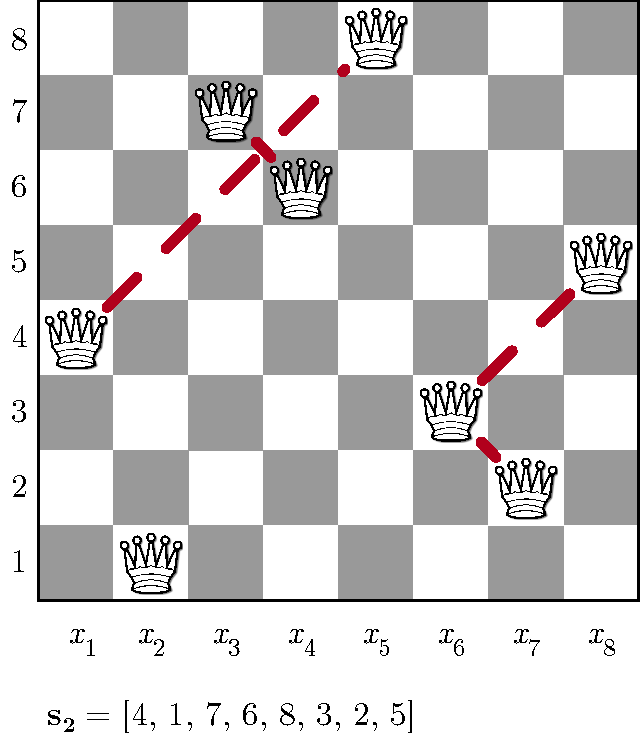
\includegraphics[width=0.4\textwidth]{"Part 2 - Search-Based Optimization/Local Search/n-queens/permutation.pdf"}}
  \end{minipage}
  \leftcaption{A state for the $n$-queens problem in the \textbf{Assignment} search space. \label{fig:nqueens-assignment}}
  \rightcaption{A state for the $n$-queens problem in the \textbf{Permutation} search space (and also in the \textbf{Assignment} one). \label{fig:nqueens-permutation}}
\end{figure}

In the \textbf{Assignment} space, horizontal and diagonal attacks have
to be taken care by the cost function $F$. In the \textbf{Permutation}
space, instead, since the search space is restricted so that two variables
cannot have the same value, also horizontal attacks are prevented by construction. In
this case, the only possible constraint violations come from the
diagonal attacks. It is easy to see that both choices are valid representations in the
sense defined above.

\subsection{Neighborhood Relation}

Given a problem $P$, an instance $I$ and a search space $S$ for it, we
assign to each element $s\in S$ a set $\mathcal{N}(s) \subseteq S$ of
neighboring states of $s$. The set $\mathcal{N}(s)$ is called the
\emph{neighborhood} of $s$ and each member $s'\in \mathcal{N}(s)$ is
called a \emph{neighbor} of $s$.

The set $\mathcal{N}(s)$ does not need to be listed explicitly, but usually
it is implicitly defined by referring to a set of possible
\emph{moves}, which define transitions between states. A move $m$
is defined by a small set of attributes that describe local
modifications of some parts of $s$. We call $s \oplus m$ the state
obtained by the application of move $m$ to state $s$. The ``locality''
of moves is the key ingredient of local search, and it has
also given the name of the whole search paradigm. Nevertheless, from
the definition above there is no implication that there is
``closeness'' in some sense among neighbors, and in fact complex
neighborhood definitions can be used as well.

The only condition that needs to be imposed on the neighborhood relation
$\mathcal{N}$ is that the search space $\mathcal{S}$ is connected
under $\mathcal{N}$. That is, every state $s$ of $\mathcal{S}$ can be
reached from any other state $s'$ by a finite-length sequence of moves
coming from $\mathcal{N}$.

Following the $n$-queens example, we consider two possible
neighborhood relations:

\begin{itemize}\itemsep 2mm
\item \textsf{Change} (\textsf{C}), for \textbf{Assignment} search space:\\
  The move \textsf{C}$\langle q,v\rangle$ assigns value $v$ to variable $x_q$.\\
  \underline{Precondition:} $x_q \neq v$.\\
%  \underline{Example:}   $[3,4,1,7,8,\textbf{4},2,1] \oplus \textsf{C} \langle 6, 1\rangle ~\rightarrow~[3,4,1,7,8,\textbf{1},2,1]$ \\
  
\item \textsf{Swap} (\textsf{S}), for \textbf{Permutation} search space:\\
The move \textsf{S}$\langle q_1,q_2\rangle$ swaps the  values assigned to variables $x_{q_1}$ and $x_{q_2}$.\\
\underline{Precondition:} $q_1\neq q_2$.\\
%\underline{Example:} $[4,\textbf{3},6,5,2,\textbf{1},8,7] \oplus \textsf{S}\langle2, 6\rangle~\rightarrow~[4,\textbf{1},6,5,2,\textbf{3},8,7]$ \\
\end{itemize}

See Figures~\ref{fig:nqueens-change} and~\ref{fig:nqueens-swap} for an example of each move, where the black arrows represent the transitions.

\begin{figure}
  \subfigures 
  \begin{minipage}{\textwidth}
    \leftfigure[t]{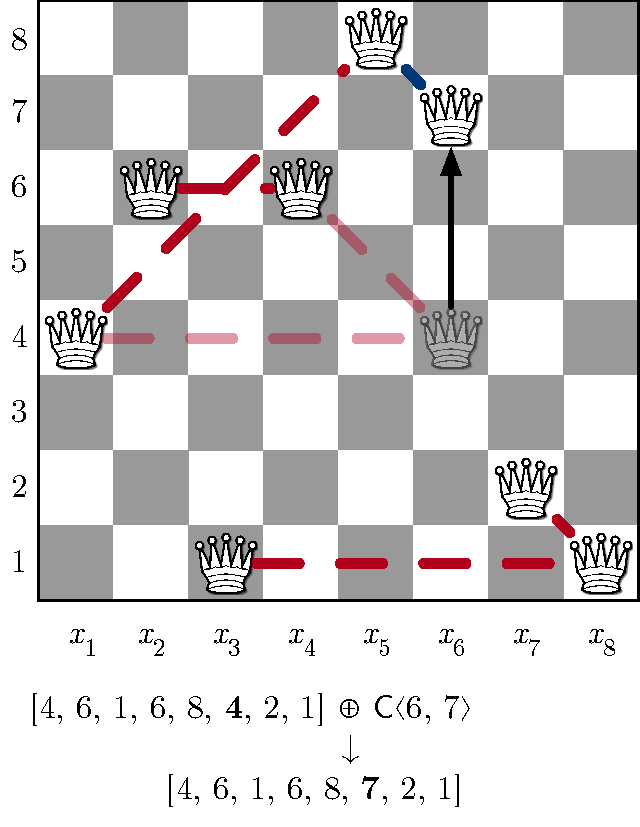
\includegraphics[width=0.4\textwidth]{"Part 2 - Search-Based Optimization/Local Search/n-queens/assignment_change.pdf"}}
    \hspace{\fill}
    \rightfigure[t]{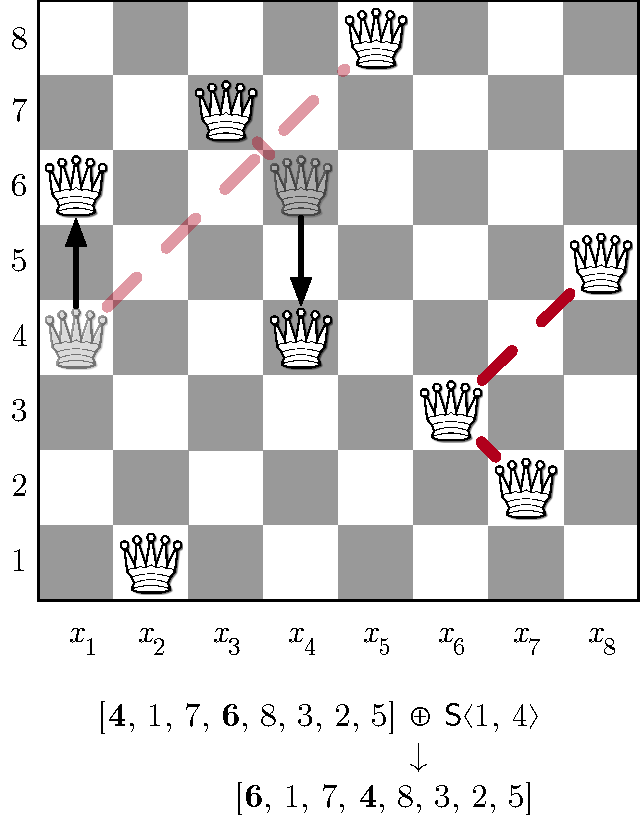
\includegraphics[width=0.4\textwidth]{"Part 2 - Search-Based Optimization/Local Search/n-queens/permutation_swap.pdf"}}
  \end{minipage}
  \leftcaption{An example of \textsf{Change} move. \label{fig:nqueens-change}}
  \rightcaption{An example of \textsf{Swap} move. \label{fig:nqueens-swap}}
\end{figure}


Notice that the \textsf{Change} neighborhood could not be applied to
the \textbf{Permutation} search space, as the moves would lead outside
the search space by duplicating some values. The \textsf{Swap}
neighborhood, instead, can also be applied to the \textbf{Assignment}
search space, but the space would not be connected under this
neighborhood, as the number of repetitions of each value does not
change upon the application of \textsf{Swap} moves, so that certain
states (with different number of repetitions) are never reached.

Nowadays there is a large body of scientific literature that shows the
effectiveness of different neighborhoods on the various problem
domains (e.g., routing and scheduling \cite{IIKM05}).
Nonetheless, the definition of a suitable neighborhood for the
specific novel problem remains a creative activity that the designers
have to undertake using their own intuition and experience. The proof
that the search space is connected under a specific neighborhood is
also a designer's task, which however is relatively easy to do for
most problems. For example, for the $n$-queens problem, for the two
proposed combinations of search space and neighborhood, it is rather
trivial to show that the search space is connected.

One of the key features of the design of the neighborhood relation is
the possibility to compute efficiently the so-called \emph{delta}
function, which is the cost difference between two neighbor states.
For example, for a \textsf{Change} move for the $n$-queens problem,
only the attacks created (resp.\ removed) by the presence in the new
(resp.\ old) position of the specific queen involved in the move needs
to be evaluated. This is easily done in linear time (with respect to
$n$). On the contrary, the full evaluation of the new state obtained
by applying the move would have a quadratic computational cost.

\subsection{Cost Function}

The selection of the move to be performed at each step is based on the
\emph{cost function} $F$ that associates to each element $s\in S$ a
value $F(s)$ that assesses the quality of the solution. For the sake
of simplicity, we assume that the value of $F$ is integer-valued and
non-negative, or in other words, that the co-domain of $F$ is the set
of natural numbers $\mathbb{N}$.

When applied to search problems, the function $F$ normally counts the
number of constraint violations, which is also known as 
\emph{distance to feasibility}. For example, in the $n$-queens
problem, the customary cost function counts the number of attacking
pairs of queens. For the state $s_1 = [4,6,1,6,8,4,2,1]$ 
represented in Figure~\ref{fig:nqueens-assignment},
we have $F(s_1) = 6$, as there are 6 pairs of queens attacking each
other $\{(x_1,x_5), (x_1,x_6), (x_2,x_4), (x_3,x_8),  (x_4,x_6),  (x_7,x_8)\}$ 
connected in the figures with red dotted lines.\footnote{Note that we count also the so-called \emph{X-ray} attacks, i.e. the ones between non consecutive queens in a row (or diagonal) of more than two of them, which by the chess rules would not attack each other.}

In the case of an optimization problem (which, without loss of
generality, is assumed to be a minimization one), $F$ typically merges
together the distance to feasibility and the objective function $f$ of
the problem.  Therefore, the cost function is typically defined as a
weighted sum, with the highest weight assigned to the distance to
feasibility, so as to give preference to feasibility over
optimality. % It seems that optimality is neglected, I would try to rephrase
%
An alternative option is to do not assign weights, but rather consider
the cost function as a pair, and perform the comparison of values in a
hierarchical way, with priority assigned to feasibility.

For some optimization problems the search space can be defined in such
a way that it represents only feasible solutions, and in those cases the cost
function normally coincides with the objective function of the problem.

In some cases, the objective function is complemented by some
auxiliary components which account for ``invisible improvements'' that
incorporate some problem knowledge that is not explicitly considered
in the objective function.  These auxiliary components might be useful
to guide the search toward promising regions of the search space.
As an example of this concept, consider the bin-packing problem for
which the objective is to minimize the number of bins and the selected
neighborhood just moves one object from one bin to another. In this
case, it could be useful to include in the cost function an auxiliary
component that favors states in which bins are filled in an unbalanced
way, rather then a situation in which objects are equally distributed
in the bids. Indeed, such an auxiliary component could create a search
trajectory composed of improving moves leading towards the removal of
one bin. % citation? Sara's phd thesis? Sect 6.3.4

Finally, it is also possible that the cost function is a surrogate of
the real objective function in the case that the latter one is
computationally expensive~\cite{KoCL11}.

\subsection{Initial Solution Selection}

An essential component of any local search procedure is the selection of
the initial solution. Typical choices are a random
generation or the use of a greedy constructive heuristic. It is also possible to use any
other search method to obtain the initial solution.

For example, for the \textbf{Permutation} space for the $n$-queens, the
random state can be obtained by creating the identity permutation
$[1,2,\dots,n]$ and then shuffling it by using the Fischer
and Yates algorithm \cite{FiYa38}.


In order to decide whether to use just a random initial state or spend
some effort to search for a greedy one, we should take into account
different aspects. In fact, on the one hand, a better initial state
would in general require less local search iterations in order to reach
high quality solutions. This saves computational time, which could be used
to perform more steps or more independent runs. On the other hand,
though, it is also possible that the greedy heuristics biases the
search toward some specific regions of the search space, so that it
might become difficult to move away toward different areas.

In some cases, the greedy procedure might be necessary in order to
obtain an initial feasible solution that a random procedure would not
reach. This behavior would allows us to avoid to be forced to include
the distance to feasibility in the cost function by finding a feasible
initial solution, thus simplifying the cost function of the local
search procedure.

% in other cases (eg bin packing) a greedy heuristic finds an initial feasible solution that represents an upper bound, which is then improved by the iterative applying the local search procedure

%For some local search techniques the construction of the initial
%solution is part of the algorithm specification, and thus it is
%required to be done in a certain way.


\subsection{Move Selection and Acceptable Criterion}

At each search step, a single move is selected. The way this selection is
performed characterizes the specific local search strategy, and we
will discuss the different options in the following sections.

However, the selection of a specific move does not inevitably imply that
the move is \emph{accepted} and performed, so that the current state is changed. On
the contrary, the move is normally subject to an acceptance condition,
which is also dependent on the specific technique under consideration.

As a general rule, moves that improve (i.e., decrease) the cost function are
accepted, but also worsening moves (i.e., increasing ones) could be accepted in specific
situations, so as to let the search move away from a \emph{local minimum}.
A local minimum is a state $s$ such that $F(s) \leq F(s')$ for all $s'
\in \mathcal{N}(s)$. When this condition holds also with a strict inequality $<$, 
we call the state a \emph{strict} local minimum. Escaping from local minima is the key issue of all local search techniques.

\subsection{Stop Criterion}\label{sec:stop-criteria}

To end the presentation of the common key elements of local search
we discuss the stop criterion, which determines when the search
is over and the best solution found that far is returned.

Many criteria have been proposed in the literature, starting from the
basic ones, typically based on the expiration of a given amount of time, 
to more complex strategies (see for example \cite[Sect.~3.2]{FrSt19}).
The basic time-expiration strategies can either refer to the wall-clock time or to more
abstract temporal measures, such as the number of iterations. The latter one has the 
advantage of not being machine dependent.

Other options might regard specific qualities of the solution reached
or the so-called \emph{stagnation} detection. That is, when no
improvement is obtained for a given number of iterations, the search is
stopped.  This way, search trials that are exploring promising paths
are let run longer than those that are stuck in regions without good
solutions or where the search is trapped.  It is also possible to
combine different criteria, by stopping the search when the first of a
set of conditions is met.  Similarly to the initial solution
selection, the stop criterion can be part of the specific technique,
therefore we will further discuss it in the following sections.
\vspace{\parskip}

Combining all the key elements presented so far, the pseudocode of a generic local search procedure is shown in
Algorithm~\ref{alg:local-search-pseudocode}.

\begin{algorithm}[ht!]
    %\renewcommand{\baselinestretch}{0.8}
    \caption{LocalSearch} \label{alg:local-search-pseudocode}   
    Parameters: SearchSpace $\mathcal{S}$, Neighborhood $\mathcal{N}$, CostFunction $F$\\   
    Output: $s_{best}$
    \begin{algorithmic}[1]
            \STATE $s \gets InitialState(\mathcal{S})$
            \STATE $s_{best} \gets s$
            \WHILE{\NOT{$StopCriterion$}}
                \STATE $m \gets SelectMove(s,\mathcal{N})$
                \STATE $\Delta F \gets F(s \oplus m) - F(s)$
                \IF{$AcceptMove(m,\Delta F)$}
                    \STATE $s \gets s \oplus m$
            \IF{$F(s) < F(s_{best})$}
                \STATE  $s_{best} \gets s$ \\
            \ENDIF
                \ENDIF
            \ENDWHILE
    \RETURN $s_{best}$
    \end{algorithmic}
\end{algorithm}

The specific definitions of the subprocedures $InitialState$, $StopCriterion$, $SelectMove$, and $AcceptMove$ characterize the specific local search technique.

%%%%%%%%%%%%%%%%%%%%%%%%%%%%%%%%%%%%%%%%%%%%%%%%%%%%%%%%%%%%%%%%%
\section{Basic Local Search Techniques}\label{sec:basics}
%%%%%%%%%%%%%%%%%%%%%%%%%%%%%%%%%%%%%%%%%%%%%%%%%%%%%%%%%%%%%%%%%

The simplest local search techniques are based on some
form of the so-called \emph{Iterative Descent} (also known as
\emph{Iterative Improvement} or \emph{Hill Climbing}).  The idea behind these 
techniques is to select at each step a move that improves the value of the objective
function or reduces the distance to feasibility, never
performing worsening moves.


\subsection{Steepest Descent}

The most well-known form of Iterative Descent is the so-called
\emph{Steepest Descent} (SD) technique. At each iteration, SD selects,
from the whole neighborhood $\mathcal{N}(s)$ of the current state
$s$, the element $s' = s \oplus m$ which has the best value of the
cost function $F$.  The SD procedure accepts the move $m$ only if it
an improving move, i.e., it decreases the value of the cost function. 
Consequently, it naturally stops as soon as it reaches a
local minimum. Therefore, assuming (as customary for combinatorial optimization) that the search space is finite and thus at least one local minimum exists, we don't need to define any other specific stop criterion.

The exhaustive exploration of the neighborhood is obtained by
enumerating the moves in a fixed order.  For example, the
\textsf{Swap} neighborhood for the $5$-queens problem, can be
enumerated in the following lexicographic order: $\{\langle 1,2\rangle, \langle
1,3\rangle, \langle 1,4\rangle, \langle 1,5\rangle, \langle
2,3\rangle, \langle 2,4\rangle, \langle 2,5\rangle, \langle
3,4\rangle, \langle 3,5\rangle, \langle 4,5\rangle\}$.

Notice that if there are two moves that lead to the same state, such as $\langle i,j\rangle$ and $\langle j,i\rangle$ in this case, only one of them should be included in order to prevent wasting time by visiting the same neighbor twice.

The enumeration of the neighborhood raises the issue of tie-breaking
in case of multiple solutions whose value of the cost function is equally good. 
The typical strategy is
to break ties in a uniform random way. That is, if there are $k$
neighbors with the same minimal cost, then each of them might be selected with
probability $1/k$.

\subsection{First-Improving Descent}


The exhaustive neighborhood exploration prescribed by the SD technique might be
rather expensive from the computational point of view. To overcome
this problem, the \emph{First-Improving Descent} (FID) technique accepts a move and moves
to a new neighbor as soon as an improving move is found. FID also
stops when there are no improving moves so that a local minimum is
detected.

In order to avoid the bias toward some specific attributes (e.g., the variables
with low indexes in the above example), the exploration of the
neighborhood should not proceed always in the same fixed order. The
simplest way to avoid such a bias is to start from a random move and
proceed onward in a circular way, by going from the last move to the first one. The procedure stops when the initial
random one is encountered again. For example, the exploration could proceed in the
following order $\{\langle 2,4\rangle,
\langle 2,5\rangle, \langle 3,4\rangle, \langle 3,5\rangle, \langle
4,5\rangle, \langle 1,2\rangle, \langle 1,3\rangle, \langle
1,4\rangle, \langle 1,5\rangle, \langle 2,3\rangle\}$ and stop as soon as an improving move has been found.

\subsection{Random Descent}

Another option to mitigate the computation burden of exhaustive neighborhood exploration 
consists in sampling the neighborhood by drawing random moves. This leads to
the \emph{Random Descent} (RD) technique that draws a (uniform) random move
at each iteration and performs it only if it is improving. 

Care should be taken to ensure that the draw is uniform. Drawing the attributes one at 
the time selecting among available values might bias the search toward moves 
that have a smaller number of possible values for the latest attributes.
For example, for the \textsf{Swap} neighborhood, drawing a random value $i$ between $1$ and 
$n-1$ and then a random value between $i+1$ and $n$, would move the queens with higher indexes move often.


The presence of a local minimum cannot be detected by RD, consequently one of
the stop criteria mentioned in Section~\ref{sec:stop-criteria} should
be used in order to decide when to finish the search.

Notice that the exhaustive exploration of the neighborhood and the random
selection can be seen as two extreme options in the trade-off between
effectiveness and efficiency of the move selection strategy. The
intermediate strategies explore exhaustively only a specific share of the
neighborhood. To this regard, a classical choice is to select randomly
a variable, but exploring all possible alternative values for that
variable and selecting the best one.


\subsection{Non-Ascent Techniques}

All the techniques discussed above can be modified by changing the
acceptance rule so that it accepts also states with equal cost value (the
so-called \emph{sideways} moves). This variant allows the search to move away
from a local minimum, but is still trapped by a strict local minimum.

In this case, we call these methods Non-Ascent techniques, rather than Descent
ones (Steepest, First-Improving, and Random). Non-Ascent
techniques have the ability to navigate through \emph{plateaux},
which are areas of the search space with equal cost, which are often
present in the landscape of many problems.

The navigation through \emph{plateaux} is often useful in reaching states from which the cost can be decreased again. On the other hand, in some cases such navigation might take a long time without producing any improvement.

\section{Discussion}\label{sec:discussion}

In this concluding section of the chapter we discuss some general
issues of local search procedures.

\subsection{Diversification vs.\ Intensification}

The main issue of local search techniques is the way they deal
with the local minima of the cost function. Even if the search
procedure employs some specific mechanism for escaping them (see, e.g., Chapter \ref{chp:simulated-annealing}),
a local minimum still behaves as a sort of \emph{attractor}.
Intuitively, when a trajectory moves away from a local minimum and
steps through a solution ``near'' to it, even though it is not allowed
to go back to the minimum itself, it still tends to move ``forward''
it (i.e., is attracted) instead of moving in an ``opposite'' direction.

For the above reason, the search procedure needs to use some form of
\emph{diversification} strategy that allows the search trajectories
not only to escape a local minimum but to move ``far'' from it thus
avoiding this sort of \emph{chaotic trapping}. 
 
On the other hand, for practical problems the landscape of the
cost function usually has the property that the value is
correlated in neighbors (and near) states.  Therefore, once a good
solution is found, it is reasonable to search in the proximity of it
for a better one. For this reason, when a local minimum is reached the
search should be in some way \emph{intensified} around it.  

In conclusion, the search algorithm should be able to balance two
sometimes conflicting objectives; it should diversify and intensify by
moving outside the attraction area of already visited local minima,
but not too far from it.  


\subsection{Smart Neighborhood Exploration}
%%%%%%%%%%%%%%%%%%%%%%%%%%%%%%%%%%%%%%%%%%%%%%%%%%%%%%%%%%%%%%%%%

Another issue in local search is the computational cost of the
exploration of the neighborhood.  Various ideas have been proposed in
the literature in order to reduce the cost of the exploration, without
penalizing the effectiveness of the search. We mention here just one
idea, known as the \emph{elite candidate list} (see, e.g., \cite[Section 3.2]{GlLa97}).

The mechanism is based on the idea of reusing the evaluations made in the
previous explorations of the neighborhood. The intuition is that if a move $m$
was good in a given solution $s$, very likely it will be still good in the neighbor 
$s' = s \oplus m'$ obtained by performing another move
$m'$.  Based on this intuition, during each neighborhood evaluation, aside selecting the best move, 
we also collect a set of other promising moves (called elite moves). 

In the subsequent iterations, the elite moves previously selected, but
not executed yet, are re-evaluated and possibly executed without
redoing the full exploration. The full exploration, and the
corresponding collection of elite moves, is performed when all
previous elite moves have been executed or discarded.



\subsection{Strategic Oscillation}
\label{sec:strategic-oscillation}
%%%%%%%%%%%%%%%%%%%%%%%%%%%%%%%%%%%%%%%%%%%%%%%%%%%%%%%%%%%%%%%%%

A strategy to overcome the risk of being trapped in a local minimum comes from the manipulation of the cost function.

The cost function of a typical local search procedure is composed by a weighted sum of a
number of components, coming from the distance to feasibility and the objective function
of the problem.  Such weights reflect the relative importance of the
various components of the objective function and the constraints.  

Even though the weights reflect the ``real'' importance of the corresponding
components, to improve effectiveness, their values might be modified during
the search procedure so as to vary the landscape of the cost function. The
temporary modification of the landscape of the cost function, known as \emph{strategic oscillation} 
can help to escape from local minima. 

The idea can be pushed further, by assigning an independent dynamic
weight not to the cost components but to each single constraint.  Such
finer grain weighting could be useful for dealing with problems with
strong asymmetries, i.e., problems in which the number of constraints
involved can be different by a large factor from variable to variable.

An analogous mechanism is based on the idea of adding to the cost
function some additional components which are specifically designed to
escape from local minima. Those extra components are chosen among the
attributes of the elements of the search space in such a way that they
get a high value on the local minimum under
consideration (see, e.g., \cite{VoTA10}).



\subsection{Complex Neighborhoods}

The last topic that we briefly discuss in this introductory chapter on local search regards the neighborhood relation. We know from the literature that for most problems there are various potential neighborhood relations available. Obviously, a state that is a local minimum for one neighborhood might not be a minimum for another neighborhood, so that the alternate use of different ones could help with the key issue of escaping local minima.

Even in cases of one single neighborhood, it is possible to consider chains of moves of length two or more that can be used as alternative relations, which would clearly have different local minima. 

In general, there are different ways to employ more than one neighborhood relation during the search. They range from considering the set-union of all neighborhoods (see, e.g., \cite{BCDS21}), to the interleaving of distinct phases in which the basic neighborhoods are used, to the use of chains of basic moves as the basic neighborhood. 

In all cases, the resulting neighborhood relation would be rather large and the exhaustive exploration problematic from the efficiency point of view. The discussion on how to explore a large neighborhood is complex and it is outside the scope of this chapter (see \cite{AEOP02}). 

\section{Exercises}

\begin{exercise}
Consider the classical \emph{graph coloring} problem, in which a given indirected graph has to be colored with a fixed number of colors avoiding that two adjacent nodes have the same color. Define a valid search space, a suitable neighborhood relation, and the cost function for this problem. 
\end{exercise}

\begin{exercise}\label{exe:flow-shop}
Consider the classical \emph{permutation flow-shop} problem, in which the order of a set of \emph{jobs} and the start and end times of their processing on a predetermined sequence of machines has to be decided. The objective is to minimize the \emph{makespan}, that is the latest completion time of a job on the last machine. Define a valid search space, one or more suitable neighborhood relations, and the cost function for this problem. 
\end{exercise}

\begin{exercise}
Consider the problem of Exercise~\ref{exe:flow-shop}, with in addition the presence of \emph{strict} due dates for the jobs, that is each job must be completely processed within its due date. How do you modify the cost function? Conversely, if the due dates are soft and the problem requires to minimize the total \emph{tardiness}, i.e., the summation of the lateness of each job, how is the cost function defined in this case?
\end{exercise}


\bibliographystyle{unsrt}
\bibliography{local_search}
